\chapter{ブラックホール、ホワイトホール、大域的因果図}

\lectureoverview{事象の地平面は局所的には何ら特別なものではなく、大域的には決定的な意味をもつ。まず地平線近傍のシュヴァルツシルト計量から出発し、ユークリッドの葉巻の類推を用いてそれを外側へとたどり、次にアリスとボブが実際に何を見ることができるかを問う。特異点と時間反転されたホワイトホール領域は、その局所的描像を永遠のシュヴァルツシルト時空へと拡大する。ペンローズのコンパクト化により、因果構造は有限で読み取れるものになる。最後の段階では、永遠の解から、重力崩壊によって作られたブラックホールへと移る。そこではニュートンの球殻定理とバーコフの定理が、接合すべき部品を与える。}

\section{地平線から無限遠まで}

十分に大きなシュヴァルツシルト地平線の近傍では、小さな実験室の範囲で曲率は弱く、動径-時間幾何は近似的に平坦である。便利な動径変数はシュヴァルツシルト座標\(r\)ではなく、一定時刻の空間的断面に沿って地平線から外向きに測った固有距離\(\rho\)である：
\begin{equation}
\rho=0 \quad\Longleftrightarrow\quad r=2GM .
\label{eq:l04-rho-horizon}
\end{equation}
便利な時間座標は無次元量
\begin{equation}
\omega=\frac{t}{4GM},
\label{eq:l04-omega}
\end{equation}
である。ここで\(c=1\)である。したがって\(\omega\)は、シュヴァルツシルト半径の2倍を単位として測ったシュヴァルツシルト時間である。

mostly-plusの規約では、地平線近傍の動径-時間計量は
\begin{equation}
ds^2\approx-\rho^2d\omega^2+d\rho^2.
\label{eq:l04-rindler}
\end{equation}
である。角方向の2次元球面は省略した。現在の議論は時間と動径距離のみに関わるからである。

\begin{figure}[htbp]
\centering
\includegraphics[width=0.72\textwidth]{lecture_04_figure_02.png}
\caption{地平線近傍の計量と再スケールされたシュヴァルツシルト時間。}
\lectureframe{00:05:46.800}
\end{figure}

式~\eqref{eq:l04-rindler}は、極座標がユークリッド平面に対して持つ関係と同じ関係をミンコフスキー時空に対して持つ。
\begin{equation}
T=\rho\sinh\omega,
\qquad
X=\rho\cosh\omega,
\end{equation}
に対して
\begin{equation}
-dT^2+dX^2=-\rho^2d\omega^2+d\rho^2.
\end{equation}
が得られる。\(\rho\)が一定の線は双曲線\(X^2-T^2=\rho^2\)であり、一方\(\omega\)は遠い過去から遠い未来へと走る。2本のヌル線\(X=\pm T\)は、縮約された図の分岐点で交わる。4次元ではその点は2次元球面を表し、未来と過去のヌル面は分岐キリング地平線を形成する。\editorialnote{交差点のみを分岐地平線と呼ぶのは、動径図における有用な略記法である。より正確には、2つの地平線の枝は分岐2次元球面上で交わる。}

\subsection{遠方領域}

シュヴァルツシルト計量の動径-時間部分は
\begin{equation}
ds^2
=-\left(1-\frac{2GM}{r}\right)dt^2
+\frac{dr^2}{1-\frac{2GM}{r}}.
\label{eq:l04-schwarzschild}
\end{equation}
である。ブラックホールから遠く、\(r\gg2GM\)では、計量は
\begin{equation}
ds^2\approx-dt^2+dr^2.
\end{equation}
に近づく。そこでは\(r\)と\(\rho\)は本質的でない加法的補正だけ異なるので、\(dt=4GM\,d\omega\)とすると、
\begin{equation}
ds^2\approx-(4GM)^2d\omega^2+d\rho^2.
\label{eq:l04-far}
\end{equation}
となる。動径方向の係数は両方の極限で単純である。変化するのは時間方向の係数である：
\begin{equation}
ds^2\approx
\begin{cases}
-\rho^2d\omega^2+d\rho^2, & \rho\ll GM,\\[3pt]
-(4GM)^2d\omega^2+d\rho^2, & \rho\gg GM.
\end{cases}
\label{eq:l04-two-limits}
\end{equation}
ホバリングする軌道に沿っては、\(d\rho=0\)である。地平線の近くでは、
\begin{equation}
d\tau=\rho\,d\omega,
\end{equation}
であるのに対し、遠方では\(d\tau\approx4GM\,d\omega=dt\)である。外部時間座標の一定の増分に対して、地平線により近く保持された時計では、経過する固有時間はますます少なくなる。

\subsection{葉巻}

時空は描きにくいので、時間的方向を通常の角度方向で置き換える。
\begin{equation}
\begin{aligned}
d\ell^2&=F(\rho)^2d\theta^2+d\rho^2,\\
F(\rho)&\sim
\begin{cases}
\rho, & \rho\to0,\\
4GM, & \rho\to\infty.
\end{cases}
\end{aligned}
\label{eq:l04-cigar}
\end{equation}
と書く。\(\rho=0\)の近くでは、これは極座標における平面である。遠方では、円周はもはや半径とともに増大しない：
\begin{equation}
C_\infty=\int_0^{2\pi}4GM\,d\theta=8\pi GM.
\label{eq:l04-cigar-circumference}
\end{equation}
したがってこの曲面は一方の端で丸みを帯び、他方の端で円柱に近づく。それは葉巻のように見える。

\begin{figure}[htbp]
\centering
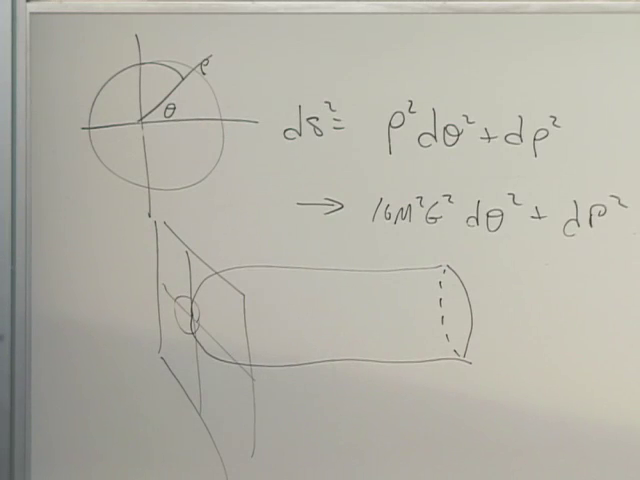
\includegraphics[width=0.74\textwidth]{lecture_04_figure_03.png}
\caption{ユークリッド的比較：極の先端が、周長\(8\pi GM\)の漸近的円柱に接合されている。}
\lectureframe{00:14:05.000}
\end{figure}

質量が大きいほど、漸近的な太さは大きくなり、先端近くの曲がりは緩やかになる。小さな穴は強く曲がった葉巻に対応し、大きな穴は広く弱く曲がった先端をもつ。これは式~\eqref{eq:l04-two-limits}における補間の描像であり、ローレンツ的ブラックホールそのものの埋め込みではない。\editorialnote{正確な幾何学的対象は、シュヴァルツシルト時間を虚時間へ解析接続することによって得られる。そのとき先端での滑らかさがユークリッド時間の周期を\(8\pi GM\)に固定する。これは後にホーキング温度を決定するのと同じスケールである。ここでは講義は視覚的類推のみを用いている。}

\section{地平線を因果的に読む}

穴の外側、\(\rho>0\)では、静止観測者は\(\rho\)が一定の双曲線に沿う。遠方では、重力に抗するのに必要な加速度はわずかである。地平線の近くでは、必要な固有加速度は際限なく増大する。世界線が未来のヌル境界を一度横切ると、そこからの未来向きの因果的信号は外部に到達できない。

\begin{classroomqa}
\audiencequestion{この図で光線は直線か？\lecturetimestamp{00:20:21}}
\lecturerresponse{別の規約が述べられない限り、動径方向の光線は\(45^\circ\)に描かれる。内向きの光線は地平線を横切る。すでに内部にある外向きの光線は、外部へと逆に横切ることはできない。}
\end{classroomqa}

\begin{classroomqa}
\audiencequestion{入射光線は地平線上にとどまるか。\lecturetimestamp{00:21:12}}
\lecturerresponse{いいえ。内向きに放たれた光線は未来の地平線を横切り、ブラックホール内部へと進み続ける。地平線の生成子自身だけが零境界上にとどまる。}
\end{classroomqa}

\subsection{ボブはアリスを観測する}

ボブが一定の半径で外側に静止してホバリングしている一方、アリスは内側へ落下する。ボブがアリスを見ることができるのは、彼女から外向きに出る光を受け取ることによってのみである。彼女が自分の時計に従って周期的に手を振っているとしよう。彼女の落下の後半に放出された信号ほど、ボブに届くまでにますます長いシュヴァルツシルト時間を要し、ボブは単位時間あたりより少ない波しか受け取らない。地平線を横切った後に放出された信号は、もはや彼のもとへ戻ることはできない。

リンドラー座標は極限的振る舞いを明らかにする。外向き零座標を
\begin{equation}
U=T-X=-\rho e^{-\omega}.
\end{equation}
と定義する。未来の地平線に近づくことは\(U\to0^{-}\)を意味し、これは固定された外部の\(\rho\)に対して\(\omega\to+\infty\)を要求する。したがって、アリスにとって有限の横断事象は、無限の外部時間へと押しやられる。連続する波の山は指数関数的に増大する間隔で到着するので、その振動数は指数関数的に赤方偏移する。\editorialnote{この零座標計算は、教室で定性的に説明された赤方偏移の数学的形式を与える。それは局所リンドラー近似のみを用いている。}

最初ボブは可視光を受け取り、次に赤外線、そして極めて長い波長の電波を受け取る。有用なのは、アリスが地平線上に永久に可視の写真としてとどまるという主張ではない。彼女は暗くなり、赤くなり、最終的には検出不可能になる。

\begin{classroomqa}
\audiencequestion{ボブはアリスが地平線の外側のちょうど一箇所で凍りついているのを見るのか。\lecturetimestamp{00:26:31}}
\lecturerresponse{古典的な外部座標による記述では、より遅い時刻に受け取られる像は、ますます地平線に近い事象から来る。極限の像はそこに凍りついているが、その放射は赤方偏移して事実上消えてしまう。量子ブラックホール物理学はまだこの説明には入っていない。}
\end{classroomqa}

\begin{classroomqa}
\audiencequestion{アリスが薄れていくにつれて、彼女は圧縮されて見えるのか。\lecturetimestamp{00:28:34}}
\lecturerresponse{はい。相対運動は外部記述において縦方向のローレンツ収縮を生じる。ここで重要な観測効果は依然として赤方偏移である。彼女の内部振動はより遅く見え、受け取られる波長は増大する。}
\end{classroomqa}

\subsection{アリスはボブを観測する}

アリスの固有時間は地平線上でも規則的であり続ける。彼女は横切った後もボブからの内向き信号を受け取り続ける。それらの信号は彼女と同じ因果的方向に従うからである。ひとたび内部に入れば、彼女は外部へ返信することはできない。地平線は一方通行であり、両側から対称に出会う壁ではない。

\begin{classroomqa}
\audiencequestion{アリスは落下して通り抜けるとき、ボブの光が青方偏移して見えるのか。\lecturetimestamp{00:30:29}}
\lecturerresponse{用いられている描像では、彼女はボブが遠ざかるのを見て、彼の信号は赤へ偏移して見える。彼女の横断において特異なことは何も起こらない。正確な振動数偏移は両方の世界線とボブがいつ放出するかに依存するので、不変な言明は、彼女が測定する振動数が正則な地平線上で有限にとどまるということである。}
\end{classroomqa}

\begin{classroomqa}
\audiencequestion{同じ因果的制限は重力子にも当てはまるのか。\lecturetimestamp{00:31:15}}
\lecturerresponse{それは光子に当てはまるのとちょうど同じように、真の重力放射にも当てはまる。未来の地平線の背後から放出された放射的擾乱は、ボブに到達することはできない。}
\end{classroomqa}

\begin{classroomqa}
\audiencequestion{アリスが落下するとき、彼女のエネルギーはブラックホールの質量と半径を増大させるのか。\lecturetimestamp{00:31:43}}
\lecturerresponse{はい。ひとたび彼女のエネルギーがブラックホールに含まれれば、その質量は増大し、そのシュヴァルツシルト半径\(R_s=2GM\)もそれに伴って増大する。動的形成の問題は、その言明を幾何学的にするであろう。}
\end{classroomqa}

\subsection{なぜ外部に依然として重力があるのか}

ブラックホールは暗いが、重力がないわけではない。定常重力場は、内部から絶えず脱出してくるオンシェル重力子の流れではない。それはすでに確立された外部幾何学である。源が変化すれば、場の変化は因果的に伝播する。遠方の観測者は、光信号が到達しうるより早くその変化を検出することはできない。

\begin{classroomqa}
\audiencequestion{重力子が脱出できないのなら、なぜブラックホールはそもそも重力を及ぼすのか。\lecturetimestamp{00:32:04}}
\lecturerresponse{静的な場はすでに外部に存在している。それを仮想重力子を用いて大まかに記述することはできるが、それらは内部からの新しい情報を運ぶ検出可能な粒子ではない。光速によって制限されるのは、重力放射を含む場の変化である。}
\end{classroomqa}

\begin{classroomqa}
\audiencequestion{仮想重力子は、場の変化は光速で伝わるという主張といかにして両立しうるのか。\lecturetimestamp{00:34:02}}
\lecturerresponse{仮想量子は摂動計算における帳簿上の要素であり、測定可能な軌道をもつ信号伝達粒子ではない。ゲージ不変な擾乱と情報は因果的に伝播する。同じ区別は、静的な電磁場と電磁放射との間にも現れる。}
\end{classroomqa}

したがって、仮想重力子は光速を超えうるという教室での言い回しは、超光速通信を意味するものとして読まれるべきではない。\editorialnote{オンシェルでない仮想粒子はオンシェルの分散関係を満たす必要はないが、それらは観測量ではなく、情報を伝達するために用いることはできない。一般相対性理論では、より簡潔な記述が可能である。すなわち、定常な外部計量は存在し、重力場の変化は因果的に伝播する。}

\section{アリスは自分の足を見ることができるか}

アリスが足から先に落下するとしよう。彼女の足は頭より先に事象の地平面を横切る。彼女が下方を見るとき、足の世界線上の同時刻の事象を見ることは決してない。光が伝わるには時間がかかるため、彼女はわずかに過去の事象にある自分の足を見る。彼女の頭が横切る前後を通じて、そのような過去の事象が連続的に続いている。彼女の体の一部が\(r=2GM\)を通過したというだけでは、局所的に不連続なことは何も起こらない。

危険な実験は、足が内側に入った後に進路を逆転させることである。頭を外側に保つには、アリスは外向きに加速しなければならない。すでに未来の地平面の向こう側にある彼女の足は、外部で静止する軌道に従うことはできない。加速系における隔たりは際限なく増大し、物質的な物体はその因果的境界を越えて剛体であり続けることはできない。彼女は足とともに自由落下するか、あるいは自分の残りの部分を外側に保とうと試みるうちに引き裂かれるかのいずれかでなければならない。

この引き伸ばしは、大きな地平面における発散する潮汐力ではない。それは、拡がりをもつ物体に対して両立しえない世界線を要求したことの帰結である。\editorialnote{十分に大きなシュヴァルツシルト地平面では、潮汐曲率は小さい。この思考実験における病的な振る舞いは、地平面における局所的な曲率特異点からではなく、試みられた加速と剛性の制約から生じる。}

\section{特異点は未来にある}

式~\eqref{eq:l04-schwarzschild}に戻ろう。外部では、
\begin{equation}
1-\frac{2GM}{r}>0,
\end{equation}
であるから、シュヴァルツシルト座標では\(t\)は時間的であり、\(r\)は空間的である。内部では、
\begin{equation}
1-\frac{2GM}{r}<0,
\end{equation}
であり、それらの座標の役割は逆転する。すなわち、\(r\)が減少する方向が時間的な方向である。これは、地平面において空間が物理的に時間に変わるという意味ではない。それは、シュヴァルツシルト図法がそこで退化し、そのラベルが内部では異なる因果的性格をもつという意味である。

真の特異点は
\begin{equation}
r=0.
\end{equation}
にある。それは、避けることのできる場所を表す垂直な世界線ではない。それは空間的な未来の境界である。アリスがブラックホール領域に入れば、未来向きの時間的またはヌルな経路はすべてそこで終わる。曲率不変量
\begin{equation}
R_{\mu\nu\rho\sigma}R^{\mu\nu\rho\sigma}
=\frac{48G^2M^2}{r^6}
\label{eq:l04-kretschmann}
\end{equation}
は\(r\to0\)として発散するが、\(r=2GM\)では有限である。\editorialnote{式~\eqref{eq:l04-kretschmann}は標準的なシュヴァルツシルト・クレッチマン・スカラーである。それは、講義で幾何学的に描かれた、正則な地平面と曲率特異点との区別を不変なものにする。}

\section{時間反転とホワイトホール}

シュヴァルツシルト計量は\(t\)に依存せず、\(dt^2\)は\(t\mapsto-t\)によって不変である。したがって、その最大拡張は時間反転に対して対称である。未来の特異点と未来の地平面に加えて、この数学的解は過去の特異点と過去の地平面を含んでいる。

アリスの落下を時間反転させよう。彼女は今や過去の特異点から現れ、過去の地平面を外向きに横切り、ボブの外部に現れる。その領域はホワイトホールと呼ばれる。それは未来のブラックホール内部からの脱出経路ではない。未来の地平面と過去の地平面は異なるヌル境界である。

\begin{classroomqa}
\audiencequestion{アリスがブラックホールの地平面を外向きに横切ることができないのなら、なぜ反転されたアリスは外に出ることができるのか。\lecturetimestamp{00:50:24}}
\lecturerresponse{彼女は未来の地平面を外向きに横切るのではない。彼女は過去の地平面を外向きに横切るのであり、それは通常の落下の時間反転にほかならない。未来のブラックホール領域には依然として外向きの因果的経路は存在しない。}
\end{classroomqa}

\begin{classroomqa}
\audiencequestion{ホワイトホールの描像では、ボブの全歴史も逆向きに走らせなければならないのか。\lecturetimestamp{00:52:15}}
\lecturerresponse{いいえ。拡張された幾何学は、ボブが外部にとどまる一方でアリスが過去の地平面から現れるような歴史を許容する。問題は数学的な整合性ではなく、過去の特異点によって表される異常な初期条件である。}
\end{classroomqa}

\begin{figure}[htbp]
\centering
\includegraphics[width=0.72\textwidth]{lecture_04_figure_04.png}
\caption{議論の間に蓄積された、交差する地平線、未来と過去の特異点曲線、および観測者の軌道からなる因果的スケッチ。}
\lectureframe{01:00:19.818}
\end{figure}

\begin{figure}[htbp]
\centering
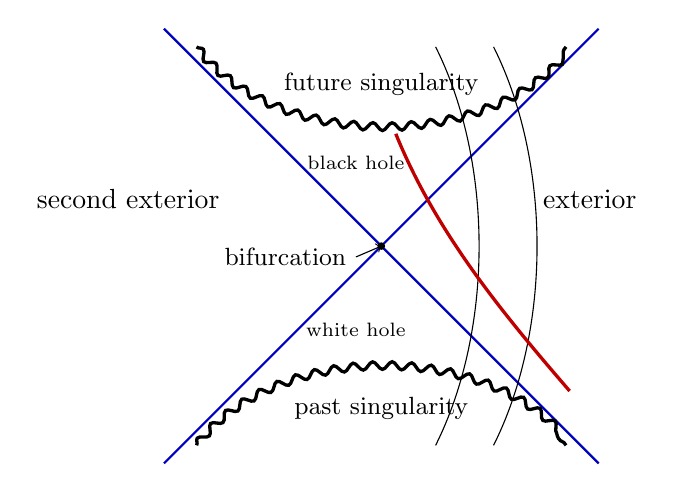
\begin{tikzpicture}[scale=0.92]
\draw[blue!75!black,thick] (-3,-3) -- (3,3);
\draw[blue!75!black,thick] (-3,3) -- (3,-3);
\draw[very thick,decorate,decoration={snake,amplitude=1.4pt,segment length=7pt}]
  (-2.55,2.75) .. controls (-1.45,1.35) and (1.45,1.35) .. (2.55,2.75);
\draw[very thick,decorate,decoration={snake,amplitude=1.4pt,segment length=7pt}]
  (-2.55,-2.75) .. controls (-1.45,-1.35) and (1.45,-1.35) .. (2.55,-2.75);
\draw (0.75,-2.75) .. controls (1.55,-1.15) and (1.55,1.15) .. (0.75,2.75);
\draw (1.55,-2.75) .. controls (2.35,-1.15) and (2.35,1.15) .. (1.55,2.75);
\draw[red!75!black,very thick] (2.6,-2.0) .. controls (1.65,-0.9) and (0.75,0.2) .. (0.2,1.55);
\fill (0,0) circle (1.5pt);
\node[above,font=\small] at (0,1.95) {future singularity};
\node[below,font=\small] at (0,-1.95) {past singularity};
\node[right] at (2.10,0.65) {exterior};
\node[left] at (-2.10,0.65) {second exterior};
\node[font=\scriptsize] at (-0.35,1.15) {black hole};
\node[font=\scriptsize] at (-0.35,-1.15) {white hole};
\node[font=\small,anchor=east] (bifurcation-label) at (-0.35,-0.15) {bifurcation};
\draw[->,thin] (bifurcation-label.east) -- (0,0);
\end{tikzpicture}
\caption{整理された非コンパクト化因果的描像。ヌル地平線は分岐面で交差し、空間的特異点は未来と過去のくさび領域にある。}
\end{figure}

\subsection{可能であることは典型的であることではない}

微視的力学は極めて良い近似で時間反転不変であるが、巨視的履歴には優先的な方向がある。爆弾は容易に爆発するが、散乱した破片が再び集まって爆弾を組み立て直すことはほとんどない。球は不安定な頂上から容易に転がり落ちるが、無作為に投げられた球がちょうどそこに静止することはほとんどない。ビリヤード球の三角形のラックは容易に散乱するが、散乱した球が自発的にラックに整列することはない。氷は熱湯の中で溶けるが、その水が新たに組み立てられた氷をほとんど吐き出すことはない。

区別はエントロピーである。低エントロピーの巨視的状態は相空間のごく小さな領域を占め、高エントロピーの巨視的状態は膨大な数の微視的配置を含む。方程式は反転した軌道を許すが、その初期微視的状態を準備するには途方もなく精密な相関が必要である。

\begin{classroomqa}
\audiencequestion{個々の散乱配置は、ちょうど時間反転した配置と同じくらい起こりにくいのではないか。\lecturetimestamp{00:56:55}}
\lecturerresponse{個別に指定された微視的状態については、その通りである。非対称性は巨視的状態を比較するときに現れる。散乱した配置は、精密に組み立てられた三角形よりもはるかに多くの微視的状態を含むので、最初の記述と両立するほとんどすべての微視的状態は巨視的には無秩序なままである。}
\end{classroomqa}

完全に組織化されたアリスを放出する白色穴は、そのようなエントロピーを下げる履歴の重力版である。それは可逆な方程式によって許されるが、極めて特別な過去を必要とする。地平線自体がエントロピーと隠れた微視的情報を担うので、アリスサイズの揺らぎは論理的に禁じられてはいない。それは圧倒的に抑制されているだけである。

\begin{classroomqa}
\audiencequestion{そのような揺らぎは量子力学的なのか、それとも熱的なのか。\lecturetimestamp{00:59:48}}
\lecturerresponse{両方の種類が寄与しうる。通常の高温系では支配的な言語は熱揺らぎである。ブラックホールでは、量子的効果と熱的効果が絡み合っている。いずれにせよ、中心的な抑制はエントロピー的なものである。}
\end{classroomqa}

\section{固有距離とペンローズコンパクト化}

大域時空を描く前に、動径に関する用語を正確にしておくべきである。固有時間とは、時間的worldlineに沿って時計が測るものである。固有距離とは、選ばれた空間的曲線に沿って局所的な物差しの連鎖が測るものである。Schwarzschildの定数\(t\)スライスに対して、
\begin{equation}
d\rho=\frac{dr}{\sqrt{1-2GM/r}}.
\label{eq:l04-proper-distance}
\end{equation}
したがって\(r\)は面積座標であり、地平線からの直接の物差し距離ではない。

さて、動径的な平坦時空から始めよう。\(t\)と\(\rho\ge0\)だけを保つ。直線\(\rho=0\)は空間的原点であり、原点に入る動径的光線は反対側の物理的側から外へ続く。これは還元された半平面上では反射として現れる。

ペンローズ図は、\(t\)と\(\rho\)のすべての有限および無限の値を、ヌル方向を保ちながら有限領域に写す。その二つの規則は次のとおりである。
\begin{enumerate}
\item 時空全体を有限領域にコンパクト化する。
\item 動径的光線を\(45^\circ\)に保つ。
\end{enumerate}
長さと通常の角度は歪められるが、因果関係は歪められない。

\begin{figure}[htbp]
\centering
\includegraphics[width=0.70\textwidth]{lecture_04_figure_06.png}
\caption{動径的Minkowski時空の完成したコンパクト化格子。無限の時間は左上と左下の端点にあり、無限の半径は右の先端に圧縮されている。}
\lectureframe{01:14:44.040}
\end{figure}

\begin{figure}[htbp]
\centering
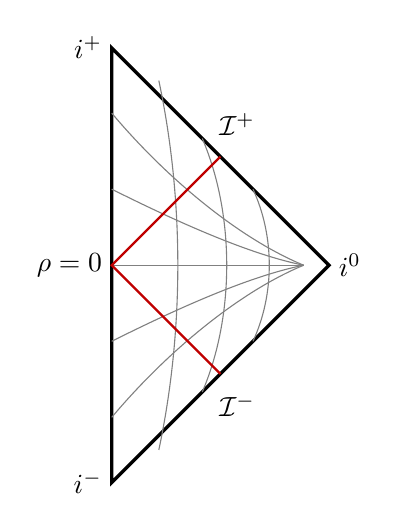
\begin{tikzpicture}[scale=0.92]
\coordinate (im) at (0,-3);
\coordinate (ip) at (0,3);
\coordinate (iz) at (3,0);
\draw[very thick] (im) -- (ip) -- (iz) -- cycle;
\draw[gray] (0,-2.1) .. controls (0.8,-1.15) and (1.8,-0.35) .. (2.65,0);
\draw[gray] (0,-1.05) .. controls (0.9,-0.6) and (1.9,-0.15) .. (2.65,0);
\draw[gray] (0,0) -- (2.65,0);
\draw[gray] (0,1.05) .. controls (0.9,0.6) and (1.9,0.15) .. (2.65,0);
\draw[gray] (0,2.1) .. controls (0.8,1.15) and (1.8,0.35) .. (2.65,0);
\draw[gray] (0.65,-2.55) .. controls (1.0,-0.9) and (1.0,0.9) .. (0.65,2.55);
\draw[gray] (1.25,-1.75) .. controls (1.7,-0.7) and (1.7,0.7) .. (1.25,1.75);
\draw[gray] (1.95,-1.05) .. controls (2.25,-0.4) and (2.25,0.4) .. (1.95,1.05);
\draw[red!75!black,thick] (1.5,-1.5) -- (0,0) -- (1.5,1.5);
\node[left] at (ip) {\(i^+\)};
\node[left] at (im) {\(i^-\)};
\node[right] at (iz) {\(i^0\)};
\node[above right] at (1.35,1.65) {\(\mathcal{I}^+\)};
\node[below right] at (1.35,-1.65) {\(\mathcal{I}^-\)};
\node[left] at (0,0) {\(\rho=0\)};
\end{tikzpicture}
\caption{有限の三角形の中の動径的Minkowski時空。赤いヌル光線は\(\mathcal{I}^-\)から入り、原点に達し、\(\mathcal{I}^+\)を通って出ていく。}
\label{fig:l04-flat-penrose}
\end{figure}

端点はそれぞれ異なる因果的意味を持つ。
\begin{equation}
\begin{aligned}
i^-&:\ \text{past timelike infinity},\\
i^+&:\ \text{future timelike infinity},\\
i^0&:\ \text{spatial infinity},\\
\mathcal{I}^-&:\ \text{past null infinity},\\
\mathcal{I}^+&:\ \text{future null infinity}.
\end{aligned}
\end{equation}
記号\(\mathcal{I}^{-}\)と\(\mathcal{I}^{+}\)はそれぞれスクリマイナス、スクリプラスと発音される。

\begin{classroomqa}
\audiencequestion{ヌル光線は歪められた格子セルすべての角を通り、したがってわずかに曲がるべきなのか。\lecturetimestamp{01:11:08}}
\lecturerresponse{完全な座標格子を正確に描けば、その交点はヌル曲線と整合するであろう。本質的な構成は共形的である。定数\(t\)および定数\(\rho\)の格子線が曲がり混み合っても、動径的ヌル方向は\(45^\circ\)に保たれる。}
\end{classroomqa}

\begin{classroomqa}
\audiencequestion{光線が原点を外れる場合、どのように描かれるのか。\lecturetimestamp{01:11:45}}
\lecturerresponse{それはゼロでない最近接距離に達し、外向きに戻る。角運動が保たれているなら、その射影された動径経路は単一の直線\(45^\circ\)である必要はない。}
\end{classroomqa}

\begin{classroomqa}
\audiencequestion{では、なぜその光線は\(45^\circ\)にないのか。\lecturetimestamp{01:12:49}}
\lecturerresponse{\(45^\circ\)の規則は動径光線に対して述べられたものである。角運動量を持つヌル光線は、その運動の一部を角度方向に使うため、\(t\)-\(\rho\)平面への射影は動径的ではない。}
\end{classroomqa}

\section{永遠のシュヴァルツシルト図}

コンパクト化された図には四つの領域がある。両側の菱形は漸近的に平坦な外部領域である。上の三角形はブラックホール内部であり、未来の空間的特異点で終わる。下の三角形はホワイトホール領域であり、過去の空間的時空特異点から始まる。これらの領域が合わさって、最大に拡張されたシュヴァルツシルト幾何学を形成する。

\begin{figure}[htbp]
\centering
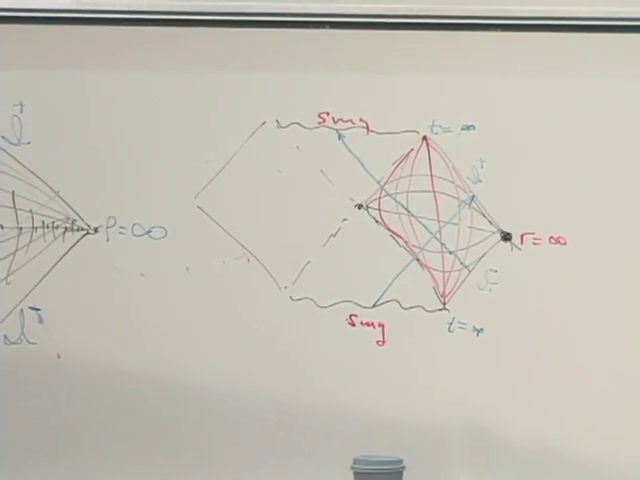
\includegraphics[width=0.74\textwidth]{lecture_04_figure_07.png}
\caption{完成した永遠のシュヴァルツシルト・ペンローズ図。特異点、事象の地平面、ヌル軌道、および一つの漸近的境界が黒板に記されている。}
\lectureframe{01:21:30.000}
\end{figure}

\begin{figure}[htbp]
\centering
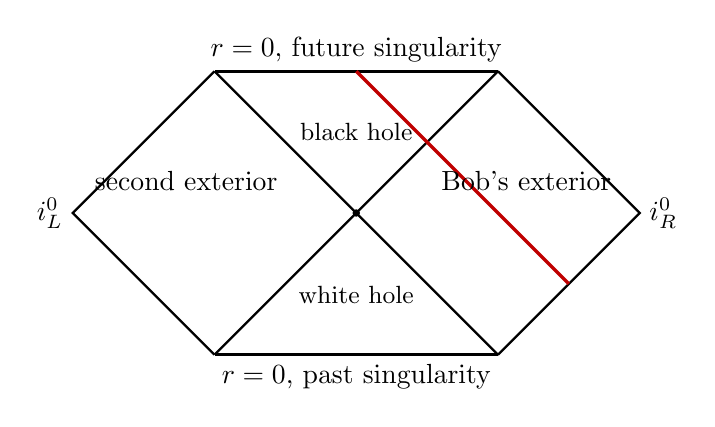
\begin{tikzpicture}[scale=0.90]
\coordinate (C) at (0,0);
\coordinate (TL) at (-2,2);
\coordinate (TR) at (2,2);
\coordinate (BL) at (-2,-2);
\coordinate (BR) at (2,-2);
\coordinate (L) at (-4.0,0);
\coordinate (R) at (4.0,0);
\draw[very thick] (TL) -- (TR);
\draw[very thick] (BL) -- (BR);
\draw[thick] (C) -- (TL) (C) -- (TR) (C) -- (BL) (C) -- (BR);
\draw[thick] (TL) -- (L) -- (BL);
\draw[thick] (TR) -- (R) -- (BR);
\draw[red!75!black,very thick] (3,-1) -- (1,1) -- (0,2);
\node[above] at (0,2) {\(r=0\), future singularity};
\node[below] at (0,-2) {\(r=0\), past singularity};
\node[font=\small] at (0,1.15) {black hole};
\node[font=\small] at (0,-1.15) {white hole};
\node at (2.4,0.45) {Bob's exterior};
\node at (-2.4,0.45) {second exterior};
\node[right] at (R) {\(i^0_R\)};
\node[left] at (L) {\(i^0_L\)};
\fill (C) circle (1.5pt);
\end{tikzpicture}
\caption{永遠のシュヴァルツシルトの四つの領域。内向きの動径光線は未来の地平面を横切り、\(r=0\)で終わる。}
\label{fig:l04-eternal}
\end{figure}

\(\mathcal{I}^-\)からの内向き動径光線は未来の地平面を横切り、特異点上で終わる。上の三角形内のすべての因果曲線も同じ運命をたどる。第二の外部領域はしばしばアインシュタイン--ローゼン橋のもう一方の口として記述されるが、それは通行可能ではない。一方の外部から他方への因果的な旅を試みると、ブラックホール領域に入り、特異点に到達する。

\begin{classroomqa}
\audiencequestion{二つの外部世界はワームホールで結ばれているのか、そしてそれを通して信号を送れるのか。\lecturetimestamp{01:22:21}}
\lecturerresponse{永遠の幾何学は適切な空間的スライス上にアインシュタイン--ローゼン橋を含むが、一方の外部から他方へ因果的信号が渡ることはない。橋はあまりに急速に窄まる。地平面に入った光でさえ未来の特異点で終わる。}
\end{classroomqa}

この図は、全時間にわたって存在してきた穴を記述している。実際の天体物理学的ブラックホールは崩壊する物質から形成される。その因果図には過去のホワイトホール特異点も第二の漸近的外部もない。その幾何学を構成するには、球殻を理解する必要がある。

\section{崩壊によるブラックホールの生成}

入射粒子からなる希薄な球殻を想像せよ。それらは光子でもよい。エネルギーは重力を生むので、十分に集中した放射パルスはブラックホールを形成しうる。崩壊前、中心領域は空の平坦時空に似ている。十分なエネルギーが圧縮された後、外部はシュヴァルツシルトに似る。課題は、動く殻を挟んでこれらの領域を接続することである。

\subsection{ニュートンの球殻定理}

全質量\(M\)の球対称ニュートン球殻に対して、重力に関するガウスの法則は
\begin{equation}
\oint \mathbf{g}\cdot d\mathbf{A}=-4\pi G M_{\mathrm{enc}}.
\label{eq:l04-gauss-gravity}
\end{equation}
球対称性により\(\mathbf{g}=g(r)\hat{\mathbf r}\)なので、
\begin{equation}
g(r)=
\begin{cases}
0, & r<R_{\mathrm{shell}},\\[4pt]
-\dfrac{GM}{r^2}, & r>R_{\mathrm{shell}}.
\end{cases}
\label{eq:l04-shell-field}
\end{equation}
内部では質量が囲まれておらず、重力場は消える。外部では、球殻は中心の点質量\(M\)と全く同じように振る舞う。内部のポテンシャルはゼロではなく一定であるが、局所的なニュートン力は残らない。\editorialnote{教室で与えられた電気力線の議論は、ガウスの法則によって正確に捉えられている。場がゼロであることとポテンシャルが一定であることの区別は、相対論で時計の規格化を比較するときに重要である。}

完全に球対称な球殻が収縮する間も、その全質量が保存される限り、結論は真のままである。内部解と外部解の境界の位置だけが変わる。

\subsection{ビルクホフの定理}

相対論的な対応物はビルクホフの定理である。すべての球対称真空領域は、局所的にシュヴァルツシルト族の一部である。中心に質量を持たない球殻に対して、
\begin{align}
ds^2_{\mathrm{inside}}&=-dT^2+dR^2+R^2d\Omega_2^2,\\
ds^2_{\mathrm{outside}}&=
-\left(1-\frac{2GM}{r}\right)dt^2
\nonumber\\
&\quad+\frac{dr^2}{1-2GM/r}
+r^2d\Omega_2^2.
\label{eq:l04-birkhoff-pieces}
\end{align}

\begin{figure}[htbp]
\centering
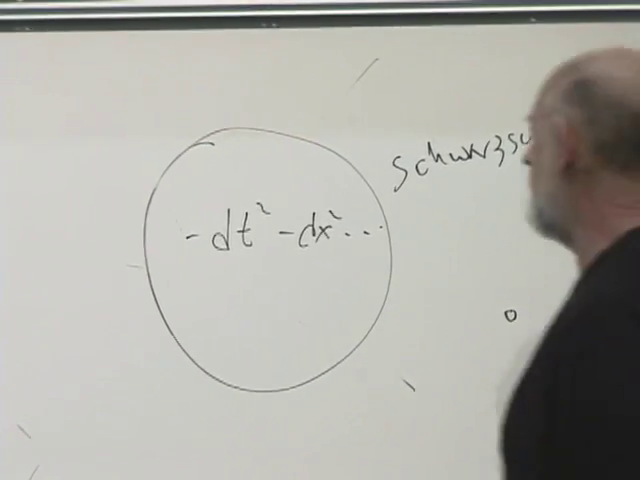
\includegraphics[width=0.74\textwidth]{lecture_04_figure_08.png}
\caption{球殻接続の黒板。円の内部は平坦時空、外部はシュヴァルツシルト解。}
\lectureframe{01:34:15.000}
\end{figure}

\begin{classroomqa}
\audiencequestion{一般相対論で球殻の外部に現れる計量は何か。\lecturetimestamp{01:33:17}}
\lecturerresponse{シュヴァルツシルト計量であり、質量パラメータは球殻の全保存質量に等しい。空の中心領域は局所的にミンコフスキー時空である。}
\end{classroomqa}

\begin{classroomqa}
\audiencequestion{殻が収縮するなら、なぜ質量パラメータは変化しないのか。\lecturetimestamp{01:34:33}}
\lecturerresponse{全エネルギーが保存されるからである。殻の半径や運動・束縛への寄与は変化しうるが、孤立した球対称系では保存される外部質量は固定されている。動く殻は、平坦領域とシュヴァルツシルト領域が接合される位置を変える。}
\end{classroomqa}

内部が平坦であることは、内部の時計が必ずしも無限遠の時計と同じ規格化をもつことを意味しない。殻をまたいだ接続により、内部時間座標が定数倍されうるし、動く殻には対応する接合条件が必要である。\editorialnote{ビルクホフの定理は各真空領域を局所的に固定する。それらの座標の大域的な関係は、殻をまたいで誘導計量と外曲率を接合することによって決まる。それらの詳細は、崩壊の構成とまったく同様に、次回の講義に先送りする。}

これで形成に必要な二つの要素がそろった。収縮する殻の内側のミンコフスキー時空と、その外側のシュヴァルツシルト時空である。殻が内側へ動くにつれ、それらの界面は世界管を描く。その管を、本来のシュヴァルツシルト半径を通り抜けて追うことにより、図~\ref{fig:l04-eternal}の非物理的な過去の半分は規則的な崩壊前領域に置き換えられ、実際のブラックホールの事象の地平面がどこで始まるかが明らかになる。
